\documentclass[11pt]{article}
\usepackage[paperwidth=172mm,paperheight=243mm,left=20mm,right=20mm,top=25mm,bottom=18mm]{geometry}
\usepackage[T1]{fontenc}\usepackage{lmodern,microtype,graphicx,xcolor,hyperref}
\pagestyle{empty}\setlength{\parindent}{0pt}
\definecolor{ink}{HTML}{122C44}\definecolor{accent}{HTML}{097F90}
\begin{document}
{\color{accent}\bfseries\sffamily\large HIGHER MATH FOR THE IMPATIENT}\par
\vspace{.8cm}
{\color{ink}\bfseries\sffamily\fontsize{31}{35}\selectfont INFORMATION\\[.13cm]GEOMETRY}\par
\vspace{.35cm}
{\color{accent}\Large When Probability Becomes Geometry}\par
\vspace{.5cm}
\begin{center}
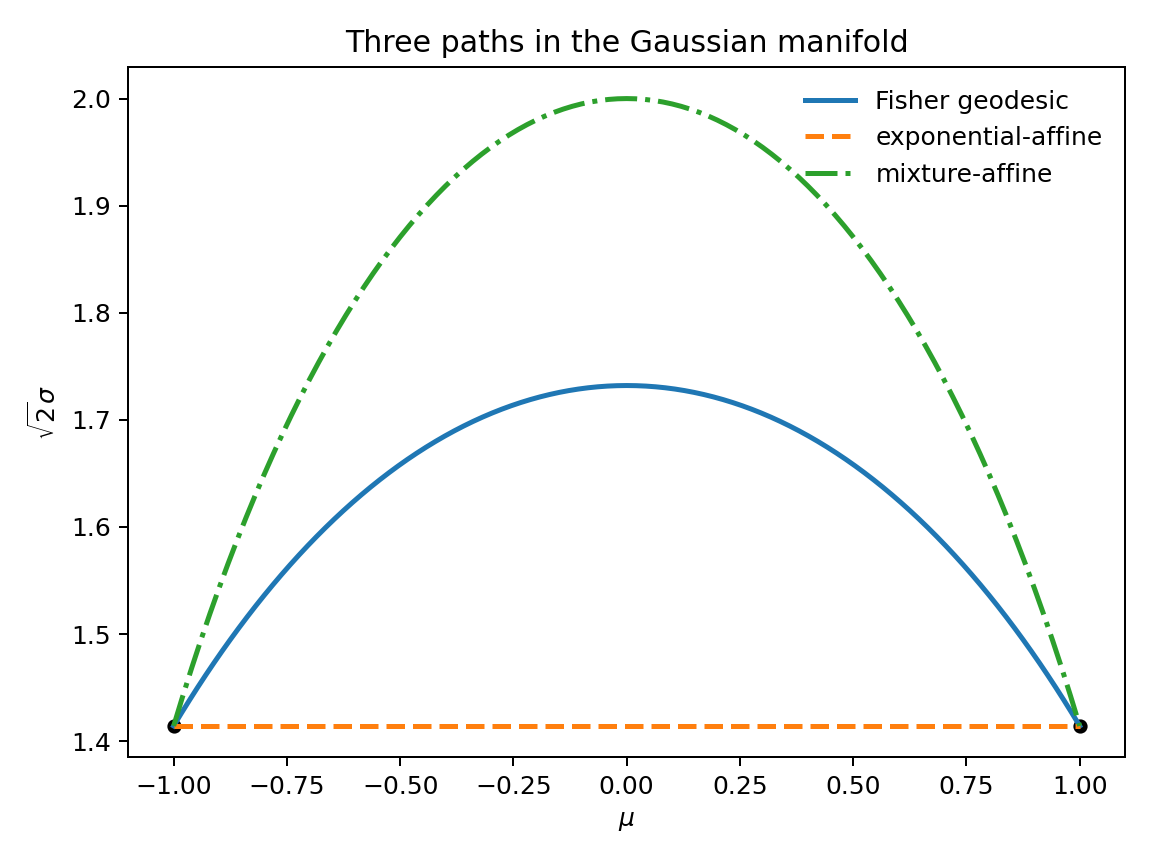
\includegraphics[width=.69\textwidth]{../figures/gaussian_three_paths.png}
\end{center}
\vspace{.5cm}
{\large\bfseries Mirco A. Mannucci}\par
HoloMathics, LLC\par
\vspace{.35cm}
{\color{accent}\bfseries WORKING RESEARCH COMPILATION -- VERSION 0.2}\par
November 2026\par
\vspace{.7cm}
\fcolorbox{accent}{white}{\begin{minipage}{.89\linewidth}
\small\textbf{Editorial note.} This compilation preserves the complete 27-page original working edition 0.1 as a PDF facsimile and appends a new, 14-page research extension with a full finite-simplex proof of \v{C}encov uniqueness, Fisher data processing, divergence-induced dual connections, exact KL projection, and natural-gradient dynamics. The original editable LaTeX source was not recovered; this is a substantive interim manuscript, not a fully integrated final edition. All new mathematics is available as editable LaTeX in IG-Lab.
\end{minipage}}\par
\vspace{.4cm}
{\small\color{ink}Book manuscript + executable mathematical laboratory + regression tests}
\end{document}
